\documentclass[12pt]{report} % Times New Roman, 12pt
%\usepackage{gscale_thesis_singlespace} % Single spaced thesis
\usepackage{gscale_thesis_doublespace} % Double spaced thesis
\usepackage{fancyheadings} % Header and footer styling
\usepackage{natbib} % Bibliography formatting
\usepackage{setspace} % Allows double spacing but skips headers/footers
\setcounter{tocdepth}{1} % Limits the TOC to chapter and section names

% Additional packages
\usepackage{graphicx} % Allows the inclusion of figures
\usepackage{subcaption} % Allows captions to be added to subfigures
\usepackage[justification=centering]{caption} % Centres caption text
\usepackage{array} % Used for table formatting
\newcolumntype{P}[1]{>{\raggedright\let\newline\\\arraybackslash\hspace{0pt}}m{#1}}
\usepackage{booktabs} % Fancy-style tables
\usepackage{longtable} % Allows for tables that are more than one page long
\usepackage{float} % Better figure placement control
\usepackage{enumerate} % Numbered lists
\usepackage[shortlabels]{enumitem} % For controlling enumerate labels
\usepackage[shortcuts]{extdash} % Allows manual hyphenation of hypenated words
\usepackage{amsmath} % Non-standard math symbols
\usepackage{amsfonts} % Extended fonts for mathematics

\usepackage[hidelinks]{hyperref} % Linking to LaTeX labels and external URLs

\numberwithin{equation}{section} % Numbers equations based on their section

% ********************************
\begin{document}
\title{Algebraic Structures in Proof Assistant Systems}
\halftitle{Algebraic Structures in Proof Assistant Systems} % 60 Characters Max. Including Spaces

\author{Akshobhya Katte Madhusudana}
\shortauthor{Akshobhya K M} % Used for page header

\dept{Department of Computing and Software}
\field{Computer Science} % What field your thesis is in (e.g. Software Engineering)

\prevdegreeone{B.Eng. (Computer Science and Engineering),\\ Bangalore University, Bangalore, India}
\prevdegreetwo{B.Eng.} % Just your degree's field

\submitdate{April 2023} % Use the month's full spelling e.g. November
\copyrightyear{2023} % Year you are submitting this, usually your graduation 
%year

\doctype{Thesis} % ``Report'' or ``Thesis'' or whatever you need
\degree{Masters of Science} % The degree you get when you submit this
\degreeabbrv{M.Sc.}
\principaladviser{Dr. Jacques Carette} % Your Supervisor
 % LaTeX variables for preface pages/headers
    
\beforepreface % Half title page, title page, declaration page   
  %\prefacesection{Lay Abstract}

A lay abstract of not more 150 words must be included explaining the key goals and contributions of the thesis in lay terms that is accessible to the general public.  % Lay Abstract
  \prefacesection{Abstract}
Algebra is the abstract encapsulation of mathematical intuition. Proof systems
can be described as an inference system that has provable statements or theorems
being their final products. It is important to study the intersection of these
powerful concepts in mathematics and computer science by carefully defining
mathematical concepts in computer language.

In this work, we study the types of algebraic structures in proof systems
especially Agda, Coq, Idris, and Lean 3 to determine the coverage of algebra in
these systems and to set the scope of our research. We contribute to the Agda
standard library, a proof assistant system, so it can be extended to other
relevant fields of algebra. We focus on commonly studied structures such as
quasigroups, loops, semigroups, rings, and Kleene algebra. These structures are
well-studied in universal algebra and have applications in various fields
including computer science, quantum physics, and mathematics. In the effort of
studying several structures with their constructs like morphisms, and direct
products and proving their properties, we analyze five problems that arise and
may not be as relevant in classical mathematics. We define more than 20
algebraic structures and add more than 40 proofs to Agda standard library. % Abstract
  %\thispagestyle{empty}
\null\vfill
\begin{center}
%\textbf{Dedications}
%\linebreak
\textsl{Your Dedication \\ Optional second line}
\end{center}
\vfill
 % Dedication
  \prefacesection{Acknowledgements}

Acknowledgements go here. % Acknowledgements
  \referencepages % Table of Contents, List of Figures, List of Tables
  \prefacesection{Notation, Definitions, and Abbreviations}

\section*{Notation}
\begin{description}[font=\rmfamily\bfseries, leftmargin=3cm, style=nextline]
	\item[$A \leq B$] A is less than or equal to B
\end{description}

\section*{Definitions}
\begin{description}[font=\rmfamily\bfseries, leftmargin=3cm, style=nextline]
	\item[Challenge] With respect to video games, a challenge is a set of goals presented to the player that they are tasks with completing; challenges can test a variety of player skills, including accuracy, logical reasoning, and creative problem solving
\end{description}

\section*{Abbreviations}
\begin{description}[font=\rmfamily\bfseries, leftmargin=3cm, style=nextline]
	\item[AI] Artificial intelligence
\end{description}
  \academicstatement{academicachievementdeclaration}
\afterpreface
  
  
  \chapter{Introduction}
Abstract algebra is the study of algebraic structure that came into existence in
the early nineteenth century as complex problems and solutions evolved in other
branches of mathematics such as geometry, number theory, and polynomial
equations. With the growing help of technology, mathematicians are more indulged
in automated reasoning. Increasing powers of computers and software tools that
help automated reasoning become useful in their research. Although the
proof systems that support first-order logic are successful, developing a tool
that supports higher-order logic is complex and requires carefully defining
mathematical objects and concepts \cite{phillips2010automated}. Proof assistant
systems act as a bridge between computer intelligence and human effort in
developing mathematical proofs. Agda, Coq, Isabelle, Lean, and Idris are some
commonly used proof assistant systems. Mathematicians use these proof assistants
to check their proof for validity, build proofs and sometimes even generate them
via proof search tools. For the scope of the thesis, we only discuss types of
algebraic structures in proof systems.

For any software system to be robust, all its dependencies must similarly be
robust. The standard libraries of these systems should support the user with
the necessary functionalities to be able to use the system easily without having to
define all functionalities. The paper \cite{BuildingDiamond} explores techniques
to generate libraries with minimum human effort. Although generated libraries
can define algebraic concepts, they are not considered "standard library" for
any proof system. For now, building standard libraries for proof systems relies
on human efforts. This led to the question of what is the current scope of
algebraic structures in the standard libraries of proof assistant systems. A
survey of the coverage of algebraic structures in the standard libraries of
proof assistant systems can help us understand which algebraic structures are
already supported by various proof assistants, and which structures are still
missing. This information can help researchers to identify gaps in existing
proof assistants and guide future development. A survey was conducted to better
understand the coverage of algebra in four proof systems Agda, Idris, Lean, and
Coq. Agda was one such system where there was better scope to contribute to the
standard library.

Agda is used by mathematicians and computer scientists for research purposes.
Contributing certain algebraic structures and theorems to Agda would help
researchers explore new domains by building upon the existing definitions and
theorems easily. The Agda standard library follows an algebra hierarchy that
starts with magma as the initial structure from which other structures are
defined. A magma is a set $S$ with a binary operation $∙$ such that, $\forall
x,y \in S, (x ∙ y) \in S$. A magma with associativity is called a semigroup.

The definitions of constructs like homomorphism and direct product are given to
us by universal algebra. Universal algebra provides a common framework by
abstracting out the specific definitions and properties of algebraic structures.
It helps us to study the commonalities of algebraic structures and define their
constructs. An algebra in universal algebra is defined as an ordered pair
$(S,F)$ where $S$ is a set and $F = (F_i:i\in I)$ is a finitary operations on A
for some indexing set $I$ \cite{sannella2012foundations}. Certain constructs
like homomorphisms, isomorphisms and direct products help us to relate different
mathematical objects and structures in a systematic and rigorous way.
Homomorphisms allow us to understand how different algebraic structures are
related to one another. Direct product, on the other hand, is a useful tool for
combining structures, such as monoids, groups, or rings, to create new and more
complex structures that retain the properties of the original structures. This
allows us to study and understand larger, more complex systems and their
properties.

\section{Research Outline}
To define the scope of our research, that is to study algebraic structures in
proof assistant systems, we capture the current coverage of algebraic structures
in the standard libraries of some commonly used proof assistant systems. As part
of the survey, we consider four libraries: The Agda standard library, the
mathematical component library for Coq, Idris 2, and mathematical library for
Lean 3. In the effort to find the coverage of algebraic structures in these
libraries, we develop a clickable table that directs to the definition of the
structure in the source code of these systems. Through the survey, we establish
our focus on contributing to the Agda standard library\footnote{I was exposed to
Agda during coursework for my Master's degree, further adding bias to choosing
Agda over other systems}.

Inspired by the ways algebraic structures are used in research, in this work we
explore capturing a select subset of them in the Agda standard library. We study
two important non-associative algebra that is quasigroup and loop structures. By
defining them with their constructs like homomorphism, monomorphism,
isomorphism, and direct product constructs, we can study their properties and
relationships in a more systematic way. We also explore various types of loops
such as bol-loop and moufang-loop and their properties. Semigroups are used in
various fields such as probability theory and formal systems. One of the most
commonly studied algebraic structures is the ring. In this thesis, we study
types of rings such as near-ring, quasi-ring, and non-associative ring. I was
exposed to Kleene Algebra in discrete mathematics course. Inspired by the
applications of Kleene algebra in finite state machines, regular expressions,
and other branches of computer science, we study Kleene algebra by providing
proof for its properties that may be used in developing other systems or
applications. By contributing to the Agda standard library, we hope that this
work will be used by others. 

As we explore capturing these structures in Agda, we encountered several
problems. In this work, we abstract out these problems into five classes:
\begin{enumerate}
\item Ambiguity in naming structures.
\item Equivalent structures that are structurally different.
\item Redundant field during structural inheritance.
\item Identical structures that can be derived in many ways in algebra hierarchy
\item Equivalent structures that are structurally the same.
\end{enumerate}
We analyze each problem and provide plausible solutions to each one of them.

\section{Thesis Outline}
Chapters 2 and 3 focus on the background information necessary for reading this
work, focusing on reviewing universal algebra and algebraic structures in Agda,
respectively. Chapter 4 is a survey on algebraic coverage in proof systems. The
next three chapters 5, 6 and 7 are dedicated to discussing the structures in
detail. Chapter 5 explores quasigroup and loop structures with their variations.
Chapter 6 discusses the properties of semigroup and ring. Chapter 7 explores
Kleene algebra, definition, construct and properties in Agda. Chapter 8
describes the various problems we faced during this work, as well as advice on
handling common issues in programming algebra in proof systems. Finally,
Chapter 9 concludes this work with notes on related future works and some
closing thoughts.
                  
        \setcounter{figure}{0}
        \setcounter{equation}{0}
        \setcounter{table}{0}
        
  \chapter{Your Chapter Title}

This is a sample chapter

If you need to use quotes, type it ``like this''.

\section{Referencing}
These are some sample references to GAMYGDALA~\citep{popescu2014gamygdala} from 
the \texttt{references.bib} file and state effects of 
cognition~\citep{hudlicka2002time} from the \texttt{references\_another.bib} 
file. These references are not in the same .bib file.

\section{Figures}
This is a single image figure (Figure~\ref{fig_singleenv}):

\begin{figure}[ht]
    \centering
    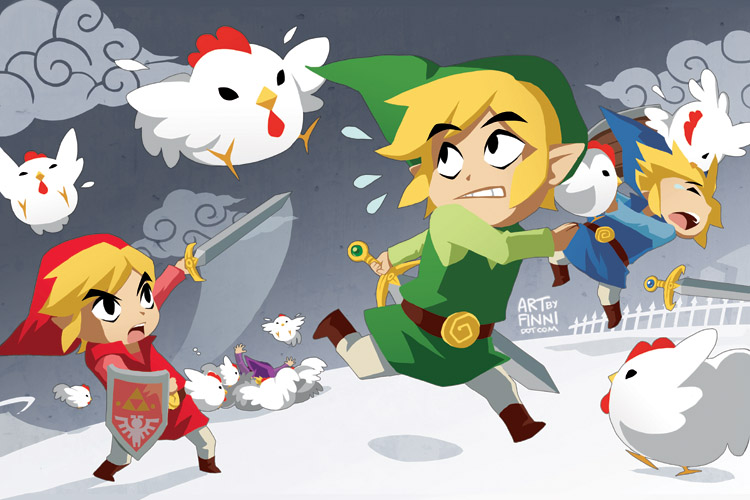
\includegraphics[width=0.6\textwidth]{figures/Sample/tumblr_static_eaceks0rfxsss8o4swscw40wo.jpg}
    \caption[Single Figure Environment Listed Title]{This is a single figure 
    environment}
    \label{fig_singleenv}
\end{figure}

This is a multi-image figure with a top (Figure~\ref{fig_multienv_1}) and bottom (Figure~\ref{fig_multienv_2}) aligned subfigures:

\begin{figure}[ht]
	\centering
	\begin{subfigure}[t]{\textwidth}
		\centering
		
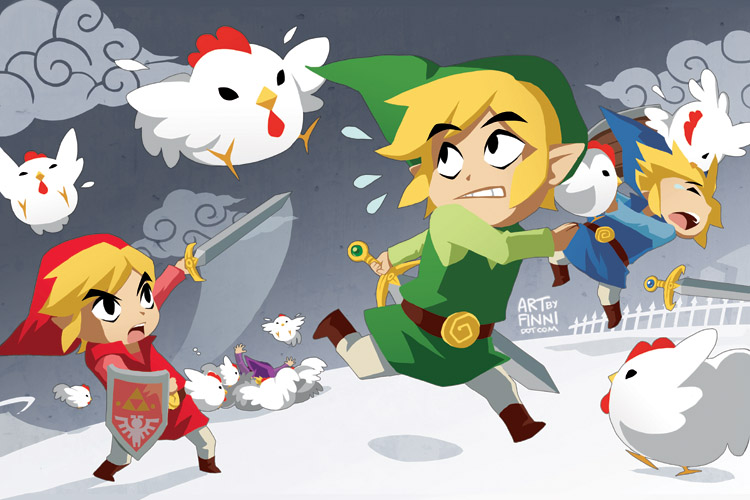
\includegraphics[width=0.7\textwidth]{figures/Sample/tumblr_static_eaceks0rfxsss8o4swscw40wo.jpg}
		\caption{Figure 1}
		\label{fig_multienv_1}
	\end{subfigure}
	~
	\begin{subfigure}[t]{\textwidth}
		\centering
		
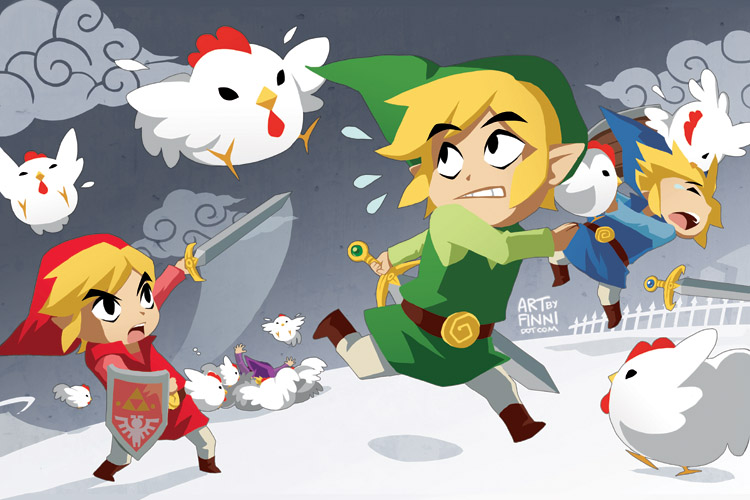
\includegraphics[width=0.7\textwidth]{figures/Sample/tumblr_static_eaceks0rfxsss8o4swscw40wo.jpg}
		\caption{Figure 2}
		\label{fig_multienv_2}
	\end{subfigure}
	
	\caption{A Multi-Figure Environment}
	\label{fig_multienv}
\end{figure}

\section{Tables}

Here is a sample table (Table~\ref{tab_sample}):

	\begin{table}[ht]
	\centering
	\begin{tabular}{ m{0.2\textwidth} m {0.1\textwidth} m{0.15\textwidth} }
		\toprule
		A & $\longleftrightarrow$ & B \\
		C & $\longleftrightarrow$ & D \\
		\bottomrule	
	\end{tabular}	
	\caption{A sample table}	
	\label{tab_sample}
\end{table}

\subsection{Long Tables}
A sample long table is shown in Appendix~\ref{appendix_b}.

\section{Equations}

Here is a sample equation (Equation~\ref{eq_lineslope}):

\begin{equation} \label{eq_lineslope}
	y = mx + b
\end{equation}                  
       \setcounter{figure}{0}
       \setcounter{equation}{0}
       \setcounter{table}{0}

  \chapter{Conclusion and Future Work}
The main of this work is to study algebraic structures in proof assistant systems. To define the scope the work we do a survey on coverage of algebraic on four proof assistant systems that are agda, idris, coq and lean 3.The thesis shows how to define a structure with some of its constructs and properties in agda. We divide this into three main chapters based on closeness of structures that is quasigroup and loop, semigroup and ring, and kleene algebra. We then analyze five problems that arises when defining algebraic structures in proof systems and give a brief overview of how it can be tackled with product family algebra. \\

In section ~\ref{contribution} we summarize the contributions of this work and how it refers to the research outline described in Chapter 1. Section ~\ref{future} discuss some extensions or future work of this work. 

\section{Summary of contributions}
\label{contribution}
Universal algebra is a well studied and evolving branch of mathematics. Proof systems are useful in automated reasoning and becoming popular in research and applications more than ever. Chapter 1 provides a overview of quantitative use of algebraic structures in proof assistant systems. We create a 'clickable' table that takes to the definition of structures in the standard libraries of the systems studied (agda, idris, lean and coq). \\

This leads to define the scope of contribution to agda standard library. Chapter 5 is dedicated to study the structures quasigroup, loop and their variations. Chapter 6 provides an overview of semigroup and ring structures with their properties and morphisms. Chapter 7 is dedicated to study of kleene algebra and it's properties in agda. Along with these structures, we define structures unital magma, invertible magma, invertible unital magma, idempotent magma, alternate magma, flexible magma, semimedial magma, medial magma, with their direct products and morphisms.\\

Our approach of defining these structures led us to analyze the problems such as ambiguity in naming, equivalent and identical structures. Chapter 8 discuss how these problems becomes more evident in proof systems that might be ignored in classical 'pen-and-paper' technique. We give an overview of how product family algebra can be used to represent and tackle these problems.

\section{Future work}
\label{future}
Our work can be extended in different ways and agda standard library is evolving with many contributions. The direct products defined in this thesis do not clearly differentiate between direct products and products and co-products. There is currently discussion on agda standard library to overcome this issue but the changes are yet to come. Product family algebra is a powerful tool to solve many problems in ontologies, cryptography and other fields. Only a brief overview of how this tool can be used is discussed in Chapter 8. A more detailed study with implementation is required to concretely say to what extent the discussed problems can be solved. This work will rely on human efforts in building strong libraries in field of abstract algebra. A more robust and reliable generative library will be helpful to reduce human efforts. 



        \setcounter{figure}{0}
        \setcounter{equation}{0}
        \setcounter{table}{0}

\begin{appendix}
    \chapter{Your Appendix}
\label{appendix_a}

Your appendix goes here.

        \setcounter{figure}{0}
        \setcounter{equation}{0}
        \setcounter{table}{0}

    \chapter{Long Tables}
\label{appendix_b}

This appendix demonstrates the use of a long table that spans multiple pages.

\begin{center}
\begin{longtable}{P{3cm}P{3cm}P{2.5cm}P{3.5cm}}
\toprule
\hline
\textbf{Col A} & \textbf{Col B} & \textbf{Col C} & \textbf{Col D} \\ \midrule

\endfirsthead
\multicolumn{4}{c}{\textit{Continued from previous page}} \\ \hline
\textbf{Col A} & \textbf{Col B} & \textbf{Col C} & \textbf{Col D} \\ \hline
\endhead
\hline \multicolumn{4}{r}{\textit{Continued on the next page}} \\
\endfoot
\hline
\endlastfoot

A & B & C & D \\ \midrule

A & B & C & D \\ \midrule

A & B & C & D \\ \midrule

A & B & C & D \\ \midrule

A & B & C & D \\ \midrule

A & B & C & D \\ \midrule

A & B & C & D \\ \midrule

A & B & C & D \\ \midrule

A & B & C & D \\ \midrule

A & B & C & D \\ \midrule

A & B & C & D \\ \midrule

A & B & C & D \\ \midrule

A & B & C & D \\ \midrule

A & B & C & D \\ \midrule

A & B & C & D \\ \midrule

A & B & C & D \\ \midrule

A & B & C & D \\ \midrule

A & B & C & D \\ \midrule

A & B & C & D \\ \midrule

A & B & C & D \\ \midrule

\hline
\end{longtable}
\end{center}

        \setcounter{figure}{0}
        \setcounter{equation}{0}
        \setcounter{table}{0}
\end{appendix}

% The bibliography is set up to allow for multiple bib files
\bibliographystyle{ACM-Reference-Format}
\bibliography{references,references_another}

\label{NumDocumentPages}

\end{document}
% ********************************
